%--------------------------------------------------------------------------
%
%                                                    ENONCE
%
%--------------------------------------------------------------------------

\noindent {\Large {\bf Questions conceptuelles }}\\[-4mm]
\begin{enumerate}
\item Les carrés et les rectangles numérotés de la figure ci-dessous représentent les positions de deux blocs à des intervalles de $0.20$s. Les blocs se déplacent vers la droite. Comparez l'accélération des deux blocs. 
\begin{center}
% 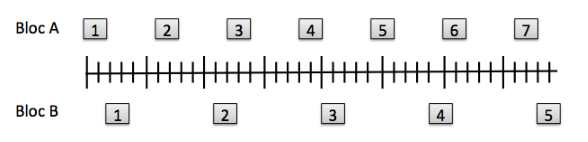
\includegraphics{figures/serie01_concept1.pdf}

 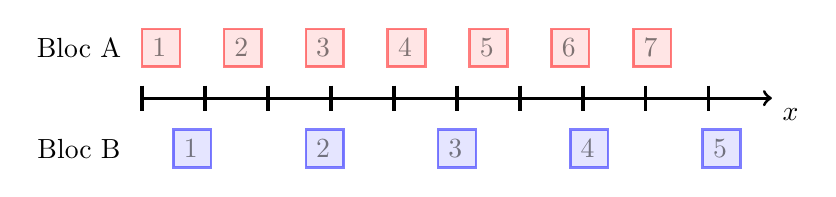
\begin{tikzpicture} [yscale=.8,xscale=.8]    
	    \draw  [- > , line width=.4mm](0,0) - -(10,0) node [below right] { $x$}; % axe horizontale
	    % XTick 
	    \draw [ line width=.4mm](0,0.2)- -(0,-0.2) ;
	    \draw [ line width=.4mm](1,0.2)- -(1,-0.2) ;
	    \draw [ line width=.4mm](2,0.2)- -(2,-0.2) ;
	    \draw [ line width=.4mm](3,0.2)- -(3,-0.2) ;
	    \draw [ line width=.4mm](4,0.2)- -(4,-0.2) ;
	    \draw [ line width=.4mm](5,0.2)- -(5,-0.2) ;
	    \draw [ line width=.4mm](6,0.2)- -(6,-0.2) ;
	    \draw [ line width=.4mm](7,0.2)- -(7,-0.2) ;
	    \draw [ line width=.4mm](8,0.2)- -(8,-0.2) ;
	    \draw [ line width=.4mm](9,0.2)- -(9,-0.2) ;
	    \draw (-1,0.8) node {Bloc A};
	    % bloc A
	    \draw [ line width=.3mm, red, fill=red!20, opacity = 0.5] (0,.5) node [above right, black] {$1$} rectangle ++(.6,.6) ;
	    \draw [ line width=.3mm, red, fill=red!20, opacity = 0.5] (1.3,.5) node [above right, black] {$2$} rectangle ++(.6,.6) ;
	    \draw [ line width=.3mm, red, fill=red!20, opacity = 0.5] (2.6,.5) node [above right, black] {$3$} rectangle ++(.6,.6) ;
	    \draw [ line width=.3mm, red, fill=red!20, opacity = 0.5] (3.9,.5) node [above right, black] {$4$} rectangle ++(.6,.6) ;
	    \draw [ line width=.3mm, red, fill=red!20, opacity = 0.5] (5.2,.5) node [above right, black] {$5$} rectangle ++(.6,.6) ;
	    \draw [ line width=.3mm, red, fill=red!20, opacity = 0.5] (6.5,.5) node [above right, black] {$6$} rectangle ++(.6,.6) ;
	    \draw [ line width=.3mm, red, fill=red!20, opacity = 0.5] (7.8,.5) node [above right, black] {$7$} rectangle ++(.6,.6) ;
	    % bloc B
	    \draw (-1,-0.8) node {Bloc B};
	    \draw [ line width=.3mm, blue, fill=blue!20, opacity = 0.5] (0.5,-1.1) node [above right, black] {$1$} rectangle ++(.6,.6) ;
	    \draw [ line width=.3mm, blue, fill=blue!20, opacity = 0.5] (2.6,-1.1) node [above right, black] {$2$} rectangle ++(.6,.6) ;
	    \draw [ line width=.3mm, blue, fill=blue!20, opacity = 0.5] (4.7,-1.1) node [above right, black] {$3$} rectangle ++(.6,.6) ;
	    \draw [ line width=.3mm, blue, fill=blue!20, opacity = 0.5] (6.8,-1.1) node [above right, black] {$4$} rectangle ++(.6,.6) ;
	    \draw [ line width=.3mm, blue, fill=blue!20, opacity = 0.5] (8.9,-1.1) node [above right, black] {$5$} rectangle ++(.6,.6) ;
  \end{tikzpicture}
\end{center}

\item Un vaisseau spatial dérive de côté dans l'espace entre P et Q. Le vaisseau n'est soumis à aucune force extérieure. A partir du point Q, le moteur du vaisseau démarre et produit une accélération constante à angle droit par rapport à PQ. Cette accélération est maintenue jusqu'à ce que le vaisseau atteigne un point R. Laquelle des trajectoires proposées représente le mieux la trajectoire du vaisseau?
\begin{center}
% 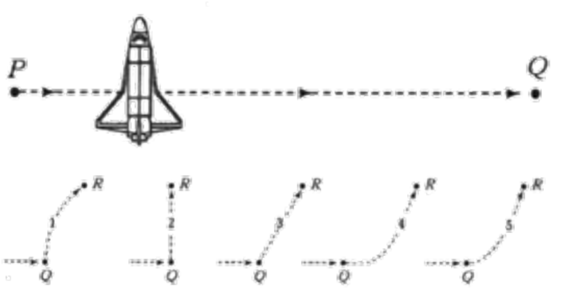
\includegraphics{figures/serie01_concept2.pdf}

\begin{tikzpicture} [scale=2]

		\draw[->, >=stealth, dashed, very thick] (-1,0) node {$\bullet$} node [above] {$P$}- -(0.95,0);
		\draw[->, >=stealth, dashed, very thick] (1,0) - -(3.95,0) ;
		\draw[->,  >=stealth, dashed, very thick] (4,0) - -(5.95,0) ;
		\node at (6,0) {$\bullet$} ;
		\node  at (6,0) [above] {$Q$};
		\node[inner sep=0pt] (shuttle) at (2,0)
   			 {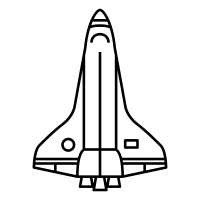
\includegraphics[width=.15\textwidth]{./figures/space-shuttle-4.png}};

		\begin{scope} [xshift=0cm,yshift=-2cm]
			\draw[->,  >=stealth, dashed, thick] (-1,0) - -(-0.05,0) ;
			\node at (0,0) {$\bullet$} ;
			\node  at (0,0) [below] {$Q$};
			\draw [->,  >=stealth, dashed, thick] (0,0) arc (180:140:1.5) ;
			\node  at (.45,1) {$\bullet$};
			\node  at (.45,1) [right] {$R$};
			\node  at (.2,.4) {$\textcircled{1}$};
		\end{scope}
		
		\begin{scope} [xshift=1.8cm,yshift=-2cm]
			\draw[->,  >=stealth, dashed, thick] (-1,0) - -(-0.05,0) ;
			\node at (0,0) {$\bullet$} ;
			\node  at (0,0) [below] {$Q$};
			\draw [->,  >=stealth, dashed, thick] (0,0) - - (0,.95) ;
			\node  at (0,1) {$\bullet$};
			\node  at (0,1) [right] {$R$};
			\node  at (.2,.4) {$\textcircled{2}$};
		\end{scope}
		
		\begin{scope} [xshift=3.4cm,yshift=-2cm]
			\draw[->,  >=stealth, dashed, thick] (-1,0) - -(-0.05,0) ;
			\node at (0,0) {$\bullet$} ;
			\node  at (0,0) [below] {$Q$};
			\draw [->,  >=stealth, dashed, thick] (0,0) - - (.45,.95) ;
			\node  at (0.5,1) {$\bullet$};
			\node  at (0.5,1) [right] {$R$};
			\node  at (.4,.4) {$\textcircled{3}$};
		\end{scope}
		
		\begin{scope} [xshift=5.2cm,yshift=-2cm]
			\draw[->,  >=stealth, dashed, thick] (-1,0) - -(-0.05,0) ;
			\node at (0,0) {$\bullet$} ;
			\node  at (0,0) [below] {$Q$};
			%\draw [->,  >=stealth, dashed, thick] (0,0) arc (-90:-50:1.5) ;
			\draw  [domain=0:0.95, samples=100,->,  >=stealth, dashed, thick] 
				plot [variable=\t]  ({\t}, {\t^2});
			\node  at (1,1) {$\bullet$};
			\node  at (1,1) [right] {$R$};
			\node  at (.2,.4) {$\textcircled{4}$};
		\end{scope}

	\end{tikzpicture}

\end{center}
\end{enumerate}

